\documentclass{beamer}
\usepackage[utf8]{inputenc}
\usepackage[spanish]{babel}
\usepackage{amsmath, amssymb, amsfonts}
\usepackage{graphicx}
\usepackage{tcolorbox}
\usepackage{hyperref}
\usepackage{caption}

\usetheme{Madrid}
\usecolortheme{default}

\title{Control de un cuadricóptero\\Modelado, linealización y control en tiempo fijo}
\author{Joan Sebastian Ramirez Sanchez\\2223948}
\institute{Introducción a la teoría de control}
\date{\today}

\begin{document}

\begin{frame}
\titlepage
\end{frame}

\begin{frame}{Contenido}
\tableofcontents
\end{frame}

\section{Introducción y modelo no lineal}

\begin{frame}{Vehículo Aéreo No Tripulado Cuadricóptero}
\begin{itemize}
    \item Plataforma de 6 grados de libertad (6-DOF) con fuerte acoplamiento no lineal.
    \item Aplicaciones: logística autónoma, inspección de infraestructura, movilidad aérea urbana.
    \item Las no linealidades surgen de las transformaciones de orientación mediante ángulos de Euler.
\end{itemize}
\vspace{0.5cm}
\textbf{Variables del sistema}
\begin{table}[h]
\small
\begin{tabular}{lll}
\hline
\textbf{Símbolo} & \textbf{Unidades} & \textbf{Descripción} \\
\hline
$\phi, \theta, \psi$ & rad & Ángulos de Euler (roll, pitch, yaw) \\
$\Omega_i$ & rad/s & Velocidad angular del rotor $i$ \\
$k_T$ & N$\cdot$s$^2$ & Constante de empuje \\
$k_D$ & N$\cdot$m$\cdot$s$^2$ & Constante de par aerodinámico \\
$I_x, I_y, I_z$ & kg$\cdot$m$^2$ & Momentos de inercia principales \\
$L$ & m & Distancia del centro al rotor \\
\hline
\end{tabular}
\end{table}
\end{frame}

\begin{frame}{Ecuaciones no lineales del sistema}
\begin{tcolorbox}[colback=brown!10!white, colframe=brown!60!black, title=No linealidades principales]
\begin{align*}
    \ddot{z} &= \frac{T}{m} \cos\phi \cos\theta - g \\
    I_x \ddot{\phi} &= \dot{\theta}\dot{\psi}(I_y - I_z) + \tau_\phi
\end{align*}
\end{tcolorbox}
\end{frame}

\section{Deducción matemática}

\begin{frame}{Fuerzas y pares generados por los rotores}
Cada rotor $i$ produce:
\begin{itemize}
    \item Empuje: $F_i = k_T\,\Omega_i^2$
    \item Par de reacción: $M_i = k_D\,\Omega_i^2$
\end{itemize}
Configuración simétrica:
\begin{align}
    T      &= k_T\sum_{i=1}^4 \Omega_i^2, \\
    \tau_\phi &= L\,k_T(\Omega_4^2-\Omega_2^2), \\
    \tau_\theta &= L\,k_T(\Omega_1^2-\Omega_3^2), \\
    \tau_\psi   &= k_D(\Omega_1^2-\Omega_2^2+\Omega_3^2-\Omega_4^2)
\end{align}
Nos centramos en el control de altitud $z$ y ángulo de alabeo $\phi$ (entradas $T$ y $\tau_\phi$).
\end{frame}

\begin{frame}{Dinámica de traslación (altitud)}
\begin{itemize}
    \item Segunda ley de Newton en el marco inercial:
    \[
    m\,\ddot{\mathbf{r}} = \mathbf{F}_{\text{empuje}} + \mathbf{F}_{\text{gravedad}}
    \]
    \item Empuje total $T$ a lo largo del eje $z$ del cuerpo. Rotación $R$:
    \[
    R = R_z(\psi)\,R_y(\theta)\,R_x(\phi)
    \]
    \item Componente vertical del empuje: $T\cos\phi\cos\theta$
    \item Gravedad: $-mg\,\hat{\mathbf{k}}$
    \item Ecuación resultante para $z$:
    \[
    \boxed{\ddot{z} = \frac{T}{m}\cos\phi\cos\theta - g}
    \]
\end{itemize}
\end{frame}

\begin{frame}{Dinámica de rotación (roll)}
\begin{itemize}
    \item Ecuaciones de Euler:
    \[
    \mathbf{I}\,\dot{\boldsymbol{\omega}} = -\boldsymbol{\omega}\times(\mathbf{I}\boldsymbol{\omega}) + \boldsymbol{\tau}
    \]
    \item Para ángulos pequeños: $p\approx\dot{\phi}$, $q\approx\dot{\theta}$, $r\approx\dot{\psi}$
    \item Primera componente (eje $x$ del cuerpo):
    \[
    I_x\,\dot{p} = q\,r\,(I_y - I_z) + \tau_\phi
    \]
    \item Sustituyendo:
    \[
    \boxed{I_x\,\ddot{\phi} = \dot{\theta}\dot{\psi}(I_y - I_z) + \tau_\phi}
    \]
\end{itemize}
\end{frame}

\begin{frame}{Modelo no lineal reducido}
\[
\begin{aligned}
\ddot{z}      &= \frac{T}{m}\cos\phi\cos\theta - g,\\[2mm]
I_x\ddot{\phi}&= \dot{\theta}\dot{\psi}(I_y - I_z) + \tau_\phi.
\end{aligned}
\]
\begin{itemize}
    \item No linealidades: productos trigonométricos y acoplamiento giroscópico.
    \item Se linealizará alrededor de un punto de equilibrio (vuelo estacionario).
\end{itemize}
\end{frame}

\section{Punto de equilibrio (hovering)}

\begin{frame}{Condiciones de vuelo estacionario}
\begin{itemize}
    \item Aceleraciones nulas: $\ddot{z}=\ddot{\phi}=\ddot{\theta}=\ddot{\psi}=0$
    \item Velocidades nulas: $\dot{z}=\dot{\phi}=\dot{\theta}=\dot{\psi}=0$
    \item Orientación horizontal: $\phi=\theta=0$ (el ángulo $\psi$ puede ser arbitrario, se toma $\psi=0$ sin pérdida de generalidad).
\end{itemize}
Sustituyendo en las ecuaciones:
\begin{align*}
    0 &= \frac{T}{m}\cos0\cos0 - g \;\Rightarrow\; T = mg\\
    0 &= \dot{\theta}\dot{\psi}(I_y-I_z) + \tau_\phi \;\Rightarrow\; \tau_\phi = 0
\end{align*}
Vectorialmente:
\[
z_e = z_0,\; \dot{z}_e=0,\; \phi_e=0,\; \theta_e=0,\; \psi_e=0,\; \dot{\phi}_e=0,\; \dot{\theta}_e=0,\; \dot{\psi}_e=0
\]
\end{frame}

\section{Linealización del sistema}

\begin{frame}{Variables de desviación}
Definimos:
\[
\delta z = z - z_e,\quad \delta \dot{z}= \dot{z},\quad \delta \phi = \phi,\quad \delta \dot{\phi} = \dot{\phi},\quad \delta T = T-mg,\quad \delta \tau_\phi = \tau_\phi
\]
Suponiendo $\theta,\psi,\dot{\theta},\dot{\psi}$ en equilibrio (cero).
Linealizando:
\begin{align*}
\delta \ddot{z} &\approx \frac{\partial}{\partial T}\Big|_{eq} \delta T + \frac{\partial}{\partial \phi}\Big|_{eq} \delta \phi + \frac{\partial}{\partial \theta}\Big|_{eq} \delta \theta \\
&= \frac{1}{m}\delta T + 0\cdot\delta\phi + 0\cdot\delta\theta = \frac{1}{m}\delta T
\end{align*}
\begin{align*}
\delta \ddot{\phi} &\approx \frac{\partial}{\partial \dot{\theta}}\Big|_{eq} \delta\dot{\theta} + \frac{\partial}{\partial \dot{\psi}}\Big|_{eq} \delta\dot{\psi} + \frac{1}{I_x}\delta\tau_\phi = \frac{1}{I_x}\delta\tau_\phi
\end{align*}
\end{frame}

\begin{frame}{Ecuaciones linealizadas y representación de estados}
Vector de estados $x = [\delta z,\; \delta\dot{z},\; \delta\phi,\; \delta\dot{\phi}]^T$, entrada $u = [\delta T,\; \delta\tau_\phi]^T$:
\[
\dot{x} = \begin{bmatrix}
0 & 1 & 0 & 0\\
0 & 0 & 0 & 0\\
0 & 0 & 0 & 1\\
0 & 0 & 0 & 0
\end{bmatrix} x +
\begin{bmatrix}
0 & 0\\
1/m & 0\\
0 & 0\\
0 & 1/I_x
\end{bmatrix} u
\]
Es decir:
\[
\dot{x} = A x + B u
\]
\end{frame}

\section{Solución del sistema linealizado}

\begin{frame}{Solución mediante matriz exponencial}
$A$ es nilpotente ($A^2=0$), por lo tanto $e^{At} = I + At$:
\[
e^{At} = \begin{bmatrix}
1 & t & 0 & 0\\
0 & 1 & 0 & 0\\
0 & 0 & 1 & t\\
0 & 0 & 0 & 1
\end{bmatrix}
\]
La solución general es:
\[
x(t) = e^{At}x(0) + \int_0^t e^{A(t-s)} B u(s)\, ds
\]
\end{frame}

\begin{frame}{Evolución temporal de los estados}
Desarrollando:
\begin{align*}
\delta z(t) &= \delta z(0) + t\,\delta\dot{z}(0) + \frac{1}{m}\int_0^t (t-s)\,\delta T(s)\,ds\\
\delta\dot{z}(t) &= \delta\dot{z}(0) + \frac{1}{m}\int_0^t \delta T(s)\,ds\\
\delta\phi(t) &= \delta\phi(0) + t\,\delta\dot{\phi}(0) + \frac{1}{I_x}\int_0^t (t-\tau)\,\delta\tau_\phi(\tau)\,d\tau\\
\delta\dot{\phi}(t) &= \delta\dot{\phi}(0) + \frac{1}{I_x}\int_0^t \delta\tau_\phi(\tau)\,d\tau
\end{align*}
\begin{figure}
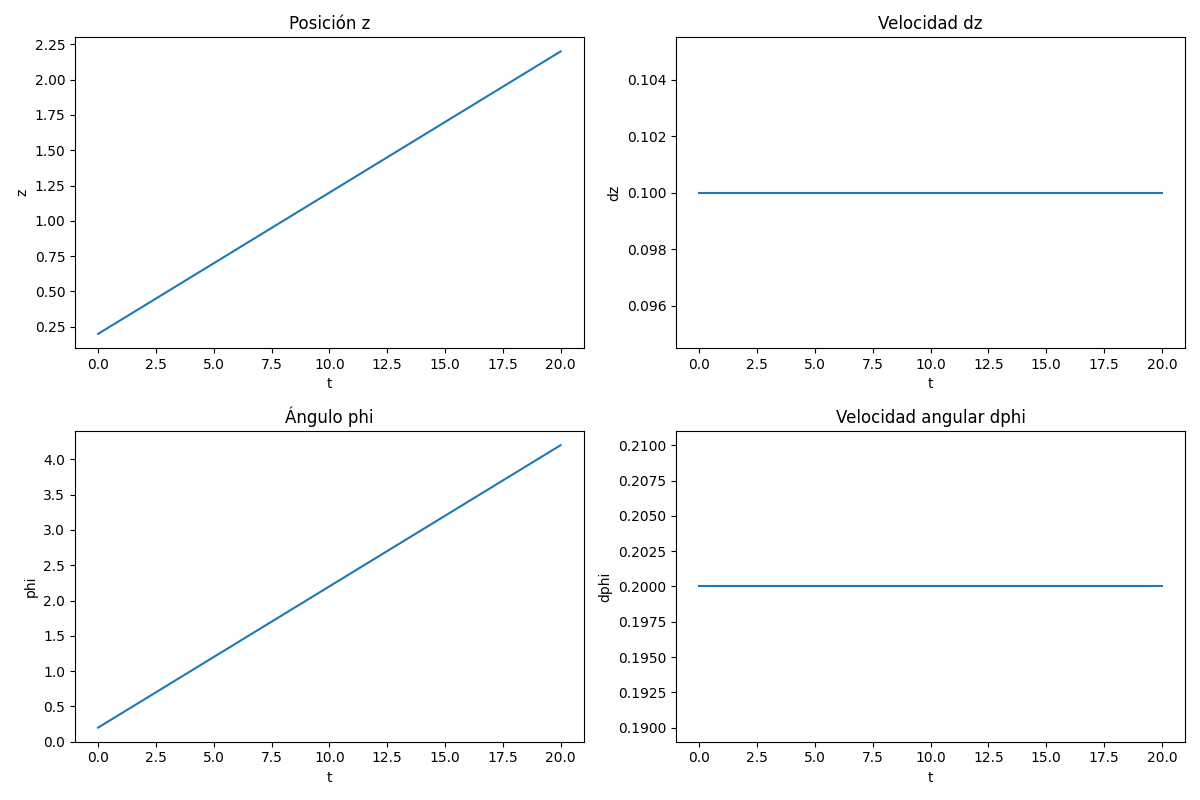
\includegraphics[width=0.7\textwidth]{graficasinforzante.png}
\caption{Evolución de los estados con entrada nula y condición inicial dada}
\end{figure}
\end{frame}

\section{Controlabilidad del sistema}

\begin{frame}{Criterio de Kalman}
Matriz de controlabilidad $\mathcal{C} = [B \;\; AB]$:
\[
AB = \begin{bmatrix}
0 & 0\\
1/m & 0\\
0 & 0\\
0 & 1/I_x
\end{bmatrix}
\]
\[
\mathcal{C} = \begin{bmatrix}
0 & 0 & 1/m & 0 & 0 & 0 & 0 & 0\\
1/m & 0 & 0 & 0 & 0 & 0 & 0 & 0\\
0 & 0 & 0 & 1/I_x & 0 & 0 & 0 & 0\\
0 & 1/I_x & 0 & 0 & 0 & 0 & 0 & 0
\end{bmatrix}
\]
Rango($\mathcal{C}$) $= 4$ $\Rightarrow$ \textbf{El sistema es controlable}.
\end{frame}

\section{Conjunto de datos admisibles}

\begin{frame}{Sin restricciones en las entradas}
\begin{itemize}
    \item No hay restricciones en las entradas $\delta T$ y $\delta\tau_\phi$.
    \item Cualquier estado inicial puede ser llevado al origen (o a cualquier estado deseado) en tiempo finito.
    \item El conjunto de datos iniciales admisibles es $\mathbb{R}^4$.
\end{itemize}
\end{frame}

\section{Control en un tiempo dado}

\begin{frame}{Control para el subsistema de altura}
Separamos en dos subsistemas independientes (altura y roll). Para la altura:
\[
\frac{d}{dt}\begin{bmatrix}x_1\\x_2\end{bmatrix} = \begin{bmatrix}0&1\\0&0\end{bmatrix}\begin{bmatrix}x_1\\x_2\end{bmatrix} + \begin{bmatrix}0\\1/m\end{bmatrix} u,\qquad u=\delta T
\]
Condiciones: $x_1(0)=\delta z_0,\; x_2(0)=\delta\dot{z}_0$; queremos $x_1(T)=0,\;x_2(T)=0$.

Usamos la fórmula (2.12) de las notas:
\[
\tilde{u}(s) = \bigl(e^{(T-s)A}B\bigr)^T G^{-1}\bigl(x_T - e^{(T-s)A}x_0\bigr),\quad G=\int_0^T (e^{tA}B)(e^{tA}B)^T dt
\]
\end{frame}

\begin{frame}{Cálculo del control óptimo en tiempo fijo}
Para el sistema doble integrador:
\[
e^{(T-s)A}B = \begin{bmatrix} T-s\\ 1\end{bmatrix}\frac{1}{m},\qquad
G^{-1} = m^2 \begin{pmatrix} \frac{12}{T^3} & -\frac{6}{T^2}\\[2mm] -\frac{6}{T^2} & \frac{4}{T} \end{pmatrix}
\]
Resultado final:
\[
\boxed{\delta T(s) = m\left[ \frac{12s-6T}{T^3}\,\delta z_0 + \frac{6s-4T}{T^2}\,\delta\dot{z}_0 \right]}
\]
Análogamente para el ángulo de roll:
\[
\boxed{\delta\tau_\phi(s) = I_x\left[ \frac{12s-6T}{T^3}\,\delta\phi_0 + \frac{6s-4T}{T^2}\,\delta\dot{\phi}_0 \right]}
\]
\end{frame}

\begin{frame}{Ejemplo numérico}
Parámetros:
\begin{itemize}
    \item $m = 0.5\ \text{kg},\quad I_x = 0.02\ \text{kg·m}^2$
    \item $T = 2\ \text{s}$
    \item $\delta z_0 = 2\ \text{m},\quad \delta\dot{z}_0 = 0.5\ \text{m/s}$
    \item $\delta\phi_0 = 0.2\ \text{rad},\quad \delta\dot{\phi}_0 = -0.1\ \text{rad/s}$
\end{itemize}
\begin{figure}
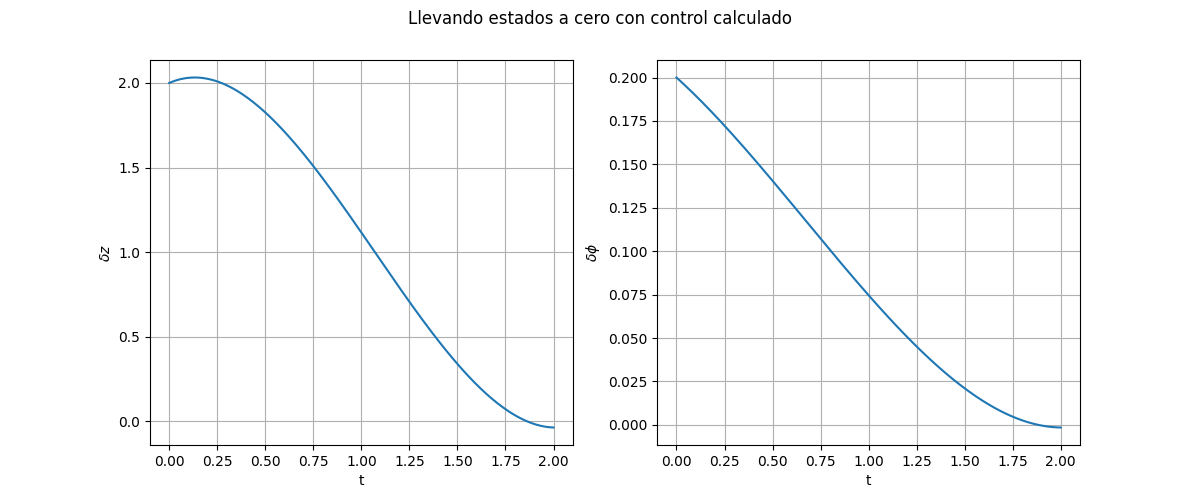
\includegraphics[width=0.8\textwidth]{graficacontorl.png}
\caption{Señales de control $\delta T(t)$ y $\delta\tau_\phi(t)$ que llevan el sistema al origen en $T=2$ segundos}
\end{figure}
\end{frame}

\begin{frame}{Conclusiones}
\begin{itemize}
    \item Se obtuvo el modelo no lineal de un cuadricóptero centrado en altitud y ángulo de roll.
    \item Se linealizó alrededor del punto de equilibrio de vuelo estacionario (hovering).
    \item El sistema linealizado es controlable (rango completo de la matriz de controlabilidad).
    \item Se diseñó una ley de control en tiempo fijo que transfiere cualquier estado inicial al origen en un tiempo $T$ prefijado.
    \item Las expresiones cerradas para $\delta T(t)$ y $\delta\tau_\phi(t)$ son fáciles de implementar.
\end{itemize}
\end{frame}

\end{document}